\documentclass[a4paper,11pt]{jsarticle}

% パッケージ
\usepackage[dvipdfmx]{hyperref}
\usepackage{pxjahyper}
\usepackage[dvipdfmx]{graphicx}
\usepackage{ascmac}
\usepackage{fancybox}
\usepackage{listings}
\usepackage{plistings}
\usepackage{color}
\usepackage{here}
\usepackage{amsmath,amsfonts}
\usepackage[subrefformat=parens]{subcaption}
\usepackage[utf8]{inputenc}
\usepackage{bm}
\usepackage{siunitx}
\usepackage{url}
% ページの周りの余白
\usepackage[top=10truemm,bottom=10truemm,left=25truemm,right=25truemm]{geometry}
% ページ番号の削除
\pagestyle{empty}

% URLの設定
\Urlmuskip=0mu  plus 10mu

% 色の定義
\definecolor{OliveGreen}{rgb}{0.0,0.6,0.0}
\definecolor{Magenta}{cmyk}{0, 1, 0, 0}
\definecolor{colFunc}{rgb}{1,0.07,0.54}
\definecolor{CadetBlue}{cmyk}{0.62,0.57,0.23,0}
\definecolor{Brown}{cmyk}{0,0.81,1,0.60}
\definecolor{colID}{rgb}{0.63,0.44,0}


\lstset{
  basicstyle={\ttfamily},
  identifierstyle={\small},
  commentstyle={\smallitshape},
  keywordstyle={\small\bfseries},
  ndkeywordstyle={\small},
  stringstyle={\small\ttfamily},
  frame={tb},
  breaklines=true,
  columns=[l]{fullflexible},
  numbers=left,
  xrightmargin=0zw,
  xleftmargin=3zw,
  numberstyle={\scriptsize},
  stepnumber=1,
  numbersep=1zw,
  lineskip=-0.5ex
}

\renewcommand{\lstlistingname}{Code}

% リンクの設定
\hypersetup{
  setpagesize=false,
  bookmarksnumbered=true,
  bookmarksopen=true,
  colorlinks=true,
  linkcolor=blue,
  citecolor=red,
}

\begin{document}
\section{目的}
  本実験では,汎用数値計算ソフトであるScilabを使用し,過渡反応についてのシュミレーションを行う.
  Scilabでのシュミレーションから,過渡反応による数値変化を確認することを目的とする.

\section{実験概要}
  \subsection{実験環境}
    実験環境を以下の表\ref{em}に示す.
    \begin{table}[H]
      \begin{center}
        \caption{実験環境}
        \begin{tabular}{|c|c|c|}  \hline 
          デバイス &  OS & ソフト \\ \hline 
          MacBookAir2019 13inch &  MacOS BigSur 11.3.1 & Scilab 6.1.0 \\ \hline
        \end{tabular}
        \label{em}
      \end{center}
    \end{table}

  \subsection{実験方法}
    本実験では,1次系伝達関数と2次伝達関数に入力する値を適当に4通り変更させ,プロットされる4つのグラフの変化から数値変化を読み取るものとする.


\section{理論}
  \subsection{Scilabとは}
    Scilabについて,以下にESI-Gropeのホームページより引用する.~\cite{ESI}
    \begin{quotation}
      Scilab/XcosはフランスのINRIA(国立情報学自動制御研究所)及びENPC(国立土木学校)で開発されたオープンソースの数値計算システムです。
      一般に公開するにあたり設立されたScilab Enterprises社が開発を担当していましたが、2017年にESI-Groupの一員となりました。
    \end{quotation}
    \begin{quotation}
      ベースとなる行列や数値計算機能だけではなく、多項式の計算や信号処理或いはそれらを視覚的に表示するプロット機能等、様々な用途に用いられています。
      そして、Windows/Linux/Mac OSの各プラットフォームに対応しています。
    \end{quotation}

  \subsection{Scilabの基本}
    \begin{figure}[H]
      \begin{tabular}{cc}
        \begin{minipage}[t]{0.48\textwidth}
          \centering
          
\includegraphics[clip,width=3cm]{picture/icon.png}
          \caption{Scilabのアイコン}
          \label{icon}
        \end{minipage} &
        \begin{minipage}[t]{0.48\textwidth}
          \centering
          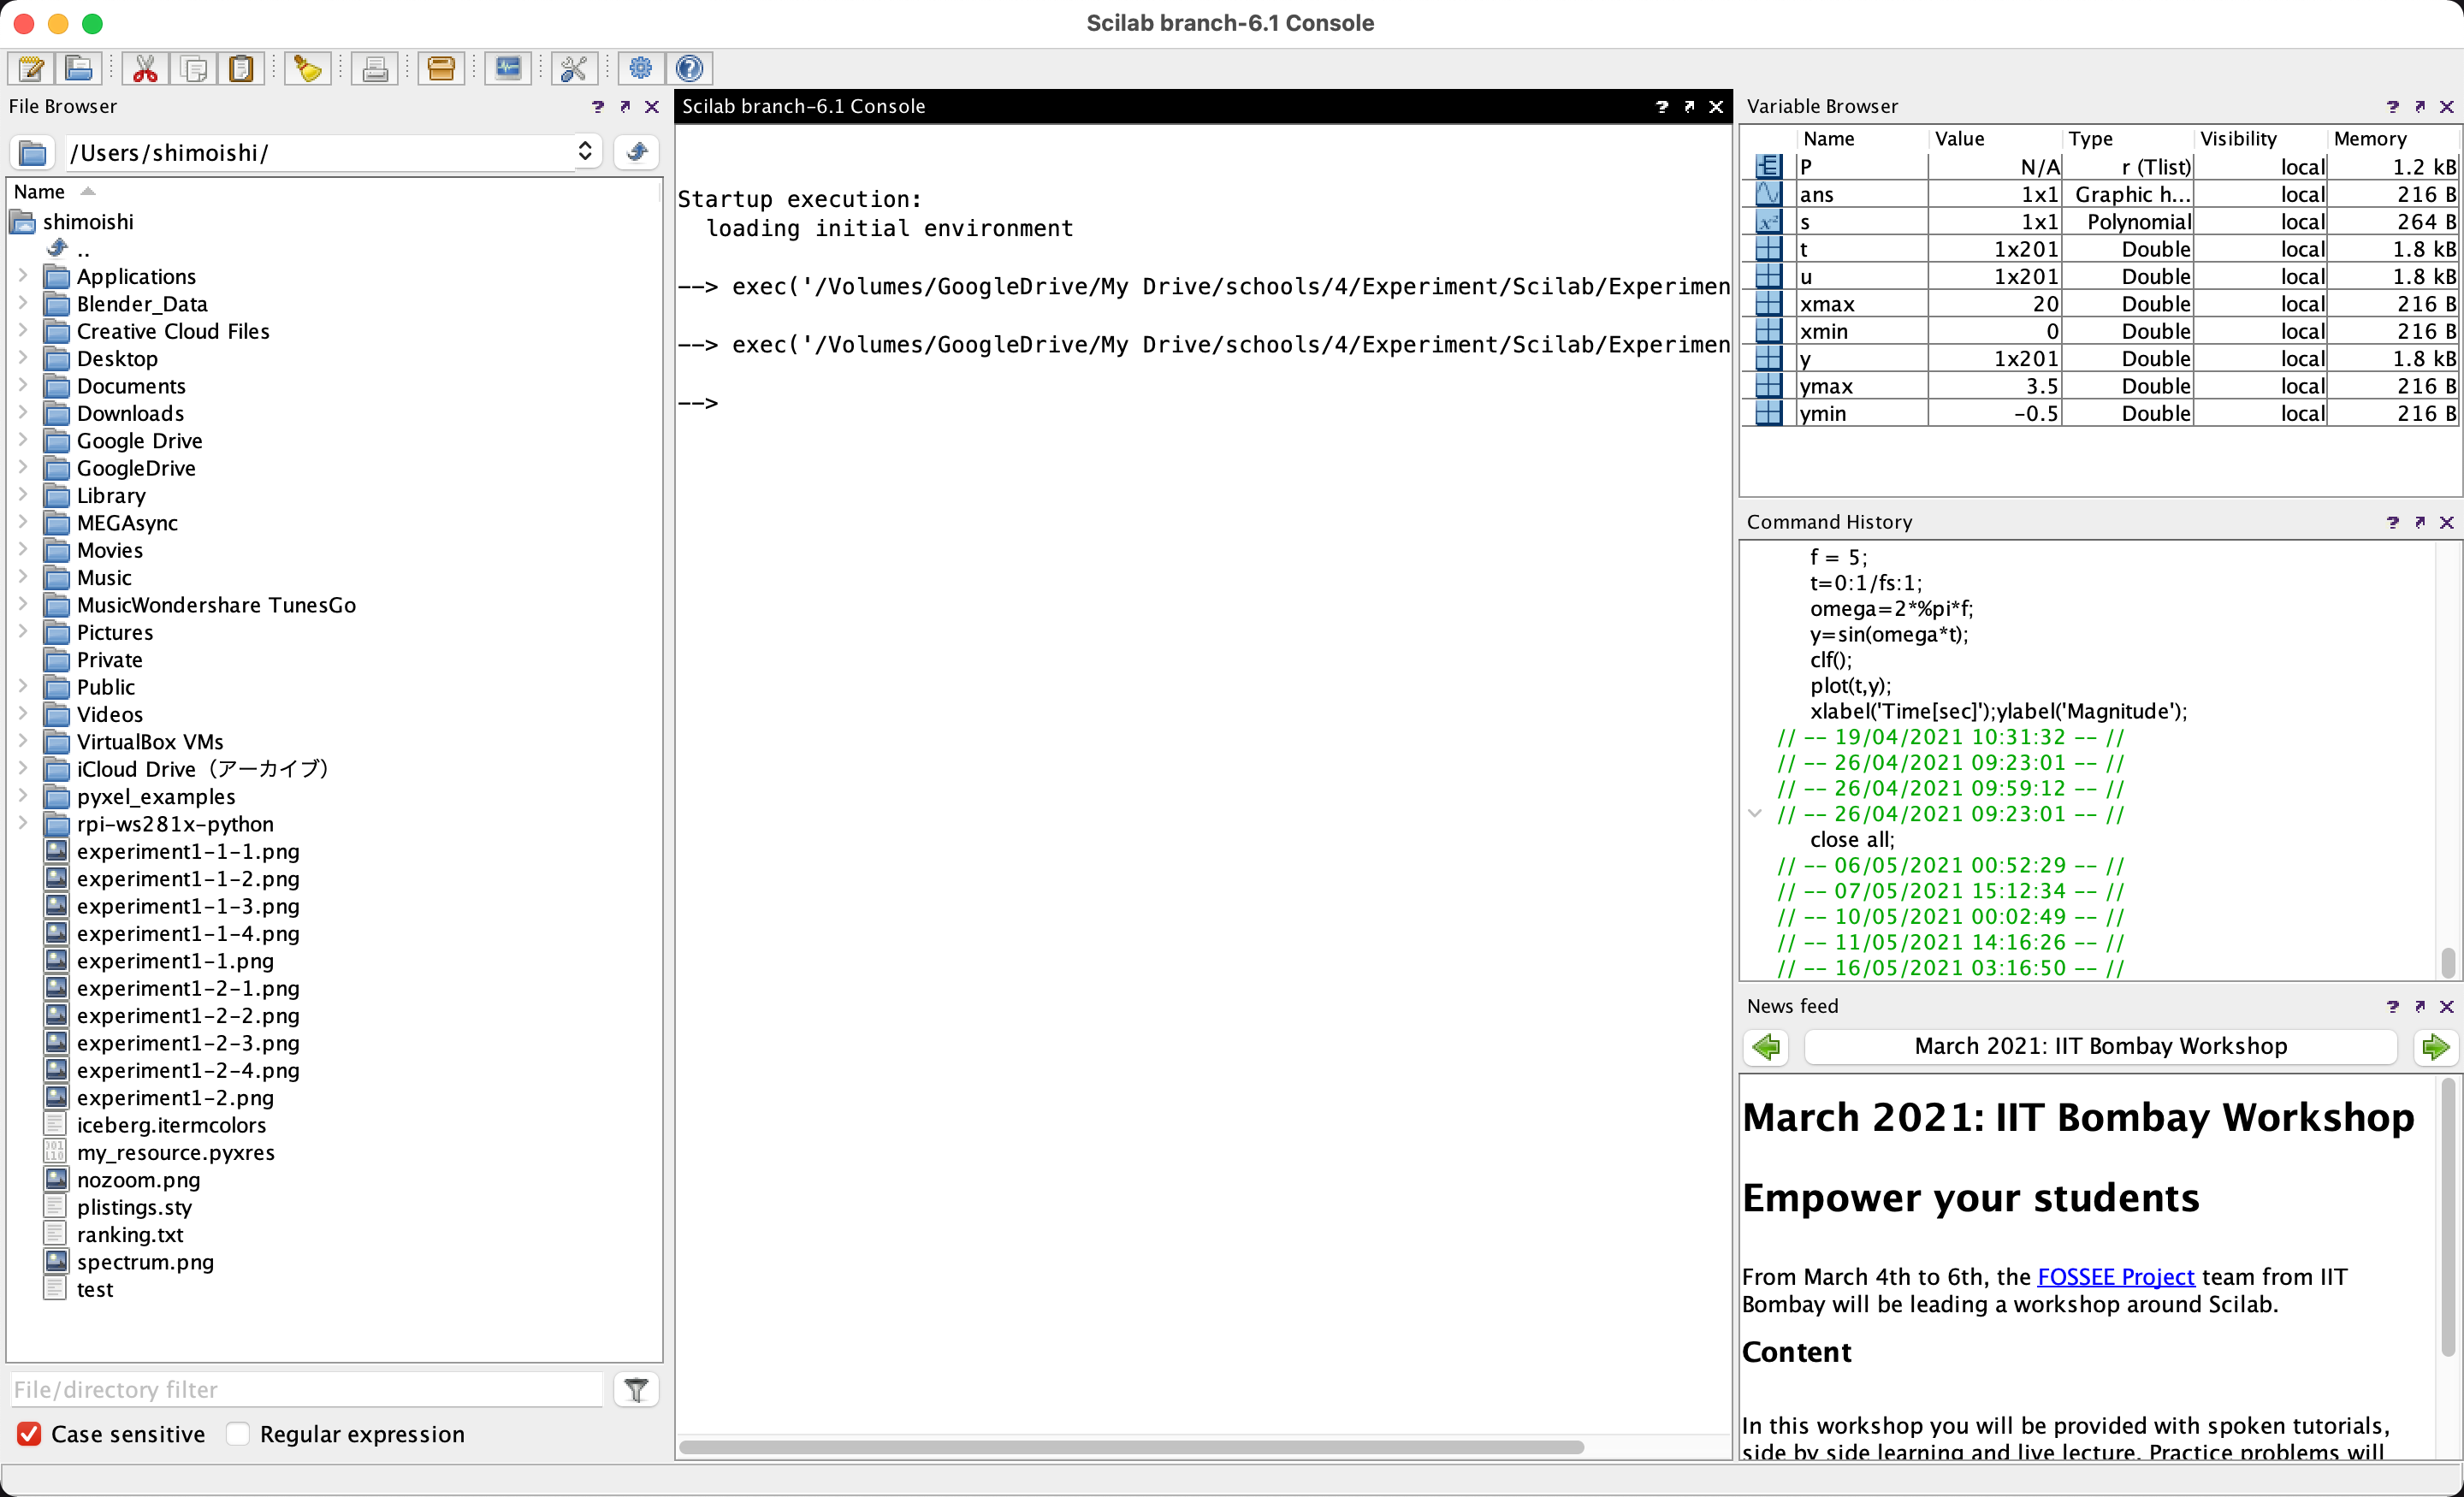
\includegraphics[clip,width=6cm]{picture/desktop.png}
          \caption{Scilabのデスクトップ}
          \label{desktop}
        \end{minipage}
      \end{tabular}
    \end{figure}
    本実験ではMacOSを使用したため,MacOS上での操作手順を示す.
      
    \subsubsection{起動・終了方法}
      Scilabを起動する際は,Scilabを起動する際は,Launchpad内のScilabのアイコン(図\ref{icon)})をクリックする.
      または,Spotlightの機能を用いて起動することもできる.
      Scilabを終了する際は,左上の×ボタンをクリックする,もしくは,
      ショートカットキー(Command + Q)から終了することができる.

    \subsubsection{数値計算}
      数値計算を行う際は,コンソールと呼ばれる領域に数値,コマンドを入力する.
      コンソールを用いる以外にも,SciNotesというウィンドウを使い数値計算をすることもできる.
      Scilabのデスクトップ(図\ref{desktop})の右上にあるアイコンから起動することができる.SciNotesはテキストエディタのように使う事ができ,
      まとまった形でプログラムを作成する事ができる.

    \subsubsection{主な関数・構文}
    Scilabを利用するにあたり,よく利用する関数や使用例を以下の表\ref{tb:command}に示す.
    \begin{table}[H]
      \centering
      \caption{よく利用される関数}
      \label{tb:command}
      \begin{tabular}{|c|c|c|} \hline
        関数 & 意味 & 注意 \\ \hline 
        \%pi & $\pi$ & \%piを付けなければならない \\ \hline
        abs & 絶対値 & $abs(-1)=1$ \\ \hline
        sqrt & 平方根 & $sqrt(2)=1.4142136$ \\ \hline
        exp & 指数関数 & $exp(1)=2.7182818$ \\ \hline
        round & 四捨五入 & $round(1.4)=1$ \\ \hline
        clear & これまでの変数をクリア & clear; これまでのデータを削除 \\ \hline
      \end{tabular}
    \end{table}
  \subsection{過渡反応}
    過渡反応~\cite{kato}とは,回路素子の値が変化や,スイッチの切り替わりにより,回路が
    ある定常状態から別の定常状態に移るまでの電流・電圧の時間的変化のことである.\\
    ここで,\\
    \begin{equation}
      G(s) = \frac{K}{Ts + 1}
      \label{1st}
    \end{equation}
    で与えられたとき,このシステムを1次系,もしくは1次遅れ系という.この式のゲイン$K$は大きくなるほど
    信号が大きく増幅されることを意味し,時定数$T$は応答の速さを示すものである.また,時刻$t=T$のとき,
    最終値の$63.2\%$に達する.つまり,式\ref{1st}にステップ入力を与えたときの出力の定常値とその$63.2\%$
    に達するまでの時間を調べることで,ゲイン$K$と時定数$T$を求めることができる.\\
    また,\\
    \begin{equation}
      G(s) = \frac{K\omega_n^2}{S^2 + 2\zeta \omega_n S + \omega_n^2}
      \label{2nd}
    \end{equation}
    で与えられたとき,このシステムを2次系,もしくは2次遅れ系という.この式の$K$はゲイン,$\zeta$は減衰係数,$\omega_n$は自然角周波数
    を表している.$\zeta > 1$は非振動的で,$0 < \zeta < 1$では振動的となる.

    
\section{実験}
  \subsection{1次系伝達関数}
    式\ref{1st}に対して適当なゲイン$K$,$T$を代入しグラフの変化を確認する.
    Scilabのソースコードを以下のCode\ref{code1}に示す.~\cite{text}\\

    \begin{lstlisting}[caption=1次系伝達関数のソースコード, label=code1]
  clear();
  s = %s;
  K = 0.5;
  T = 3;
  P = syslin('c', K/(T*s+1));
  t = 0:0.1:20;
  u = ones(t);
  y = csim(u,t,P);
  xmin = 0; xmax = 20; ymin = -0.5; ymax = 3.5;
  scf(0);

  plot2d(t,u,style=color(0,0,255),rect=[xmin ymin xmax ymax]);

  plot2d(t,y,style=color(255,0,0),rect=[xmin ymin xmax ymax]);

  xtitle('Step Response', 'time[s]', 'u, y')
  xgrid();

  //save file as PNG
  xs2png(0, 'experiment1-1-4.png')

    \end{lstlisting}

    また,以下の図\ref{kadai1_G}にそれぞれ値を変化させたグラフを示す.
    \begin{figure}[H]
      \begin{tabular}{cc}
        \begin{minipage}[t]{0.48\textwidth}
          \centering
          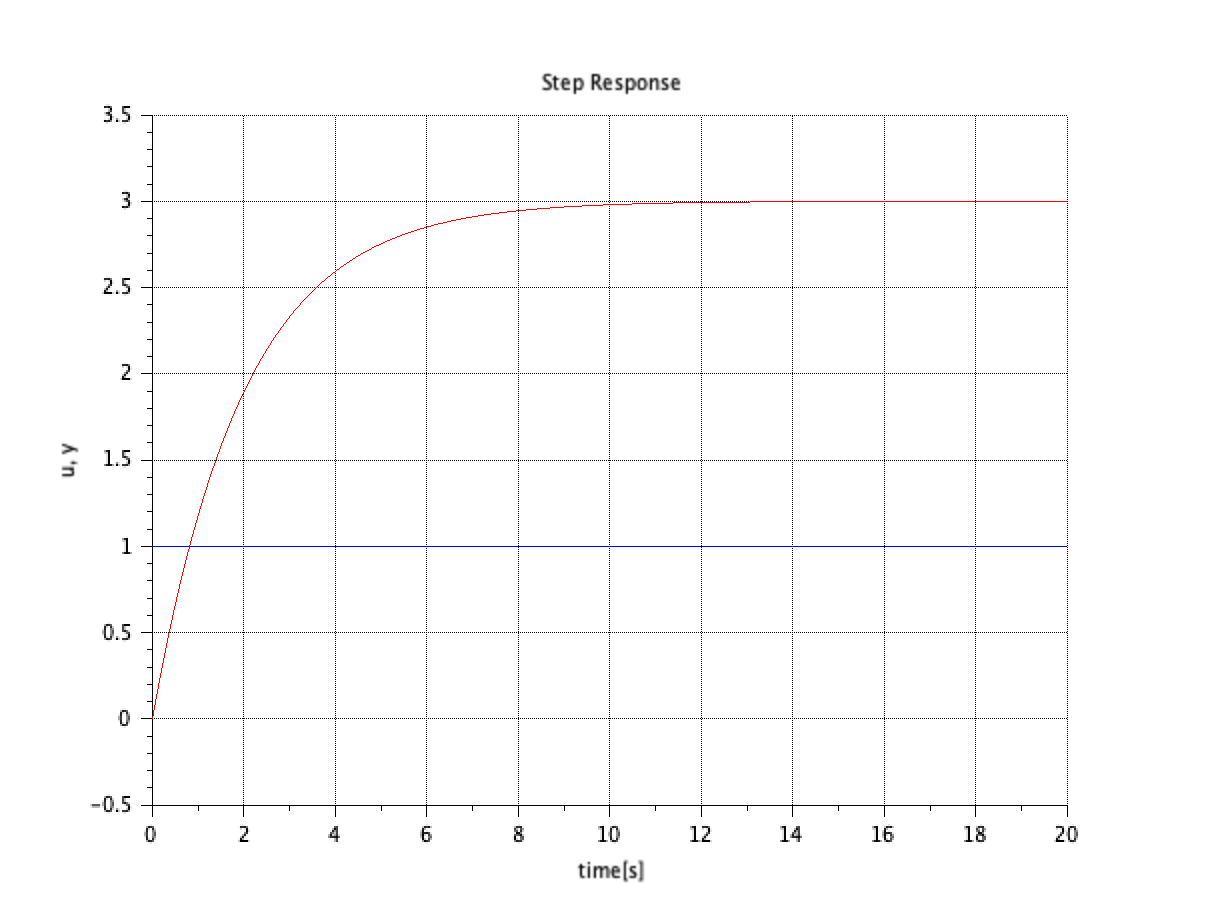
\includegraphics[clip,width=9cm]{picture/experiment1-1-1.png}
          \subcaption{$K=3, T=2$のときのグラフ}
          \label{G1-1}
        \end{minipage} &
        \begin{minipage}[t]{0.48\textwidth}
          \centering
          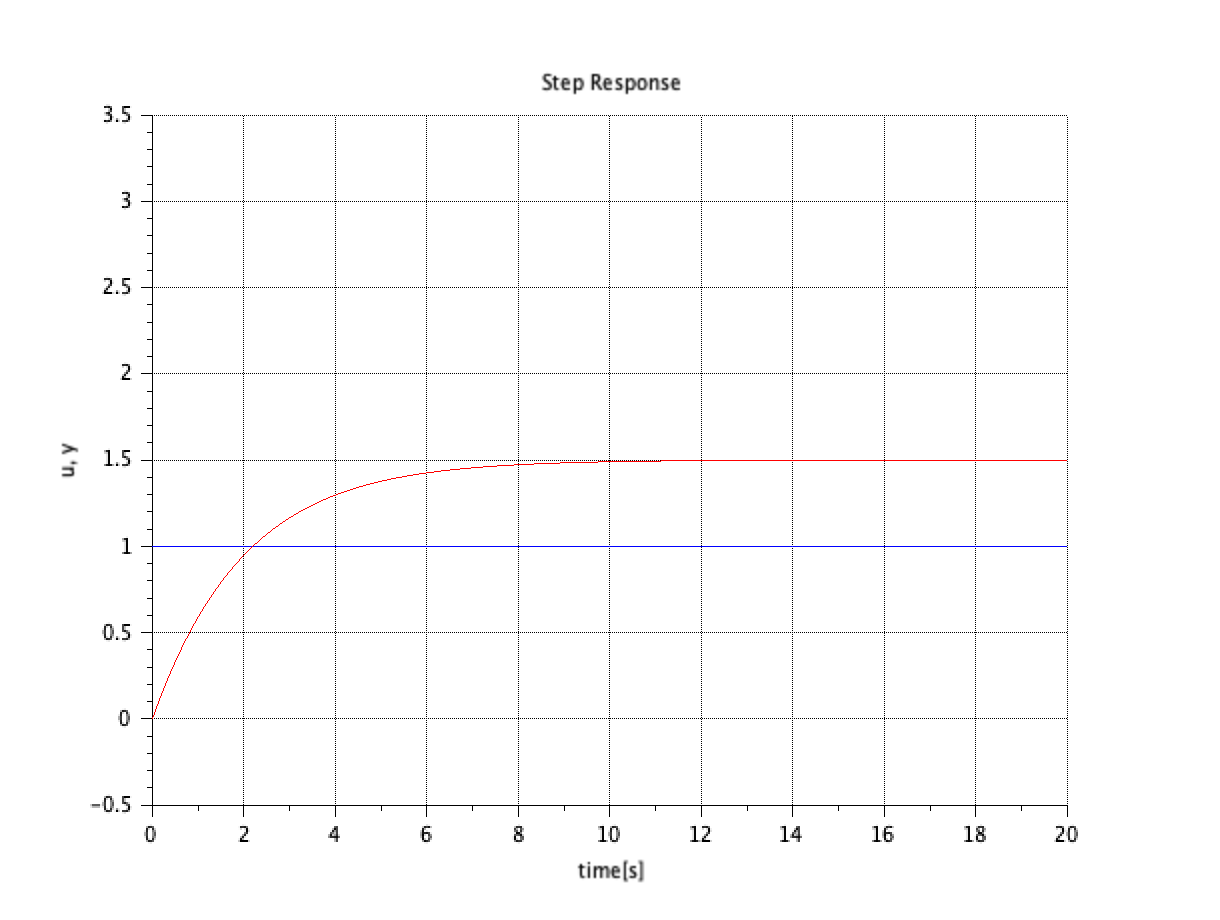
\includegraphics[clip,width=9cm]{picture/experiment1-1-2.png}
          \subcaption{$K=1.5, T=2$のときのグラフ}
          \label{G1-2}
        \end{minipage} \\
        \begin{minipage}[t]{0.48\textwidth}
          \centering
          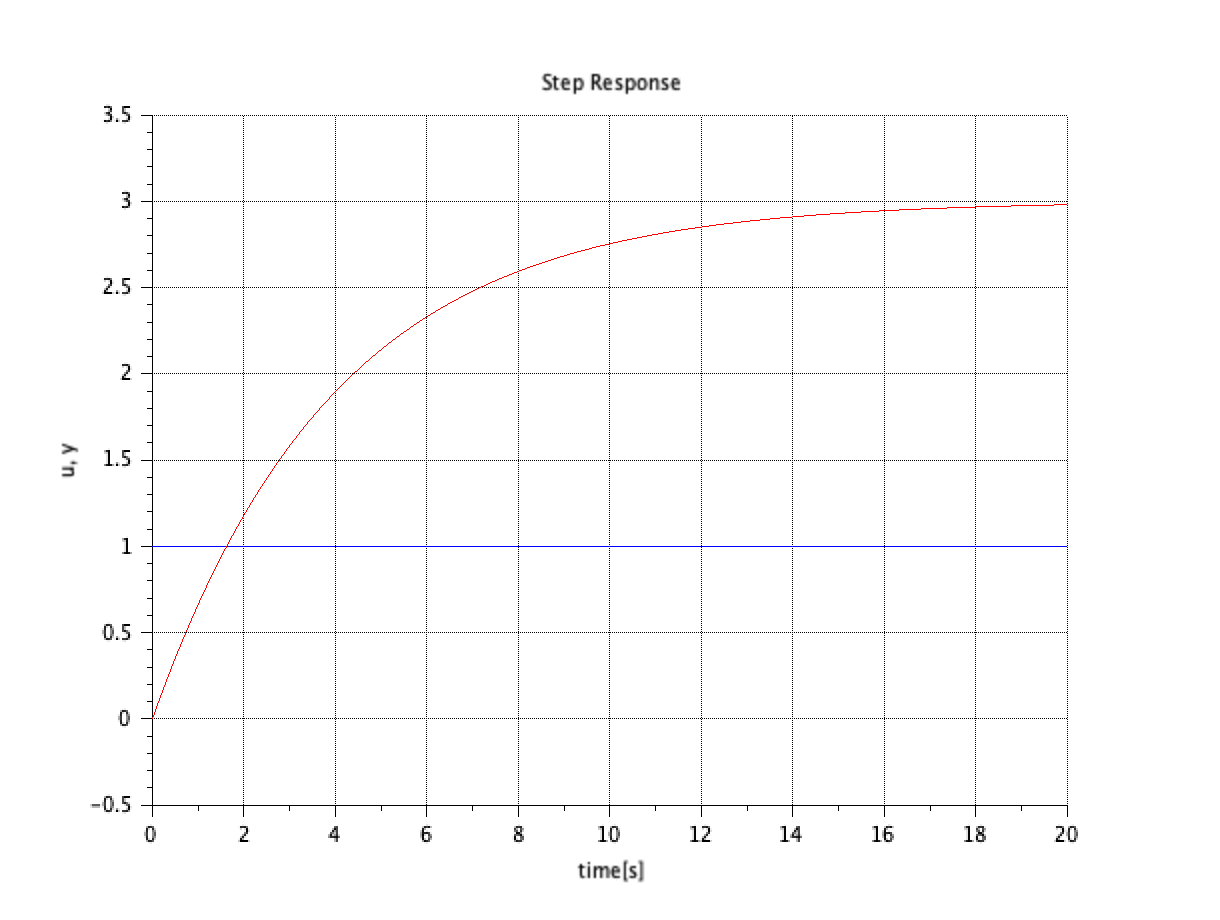
\includegraphics[clip,width=9cm]{picture/experiment1-1-3.png}
          \subcaption{$K=3, T=4$のときのグラフ}
          \label{G1-3}
        \end{minipage} &
        \begin{minipage}[t]{0.48\textwidth}
          \centering
          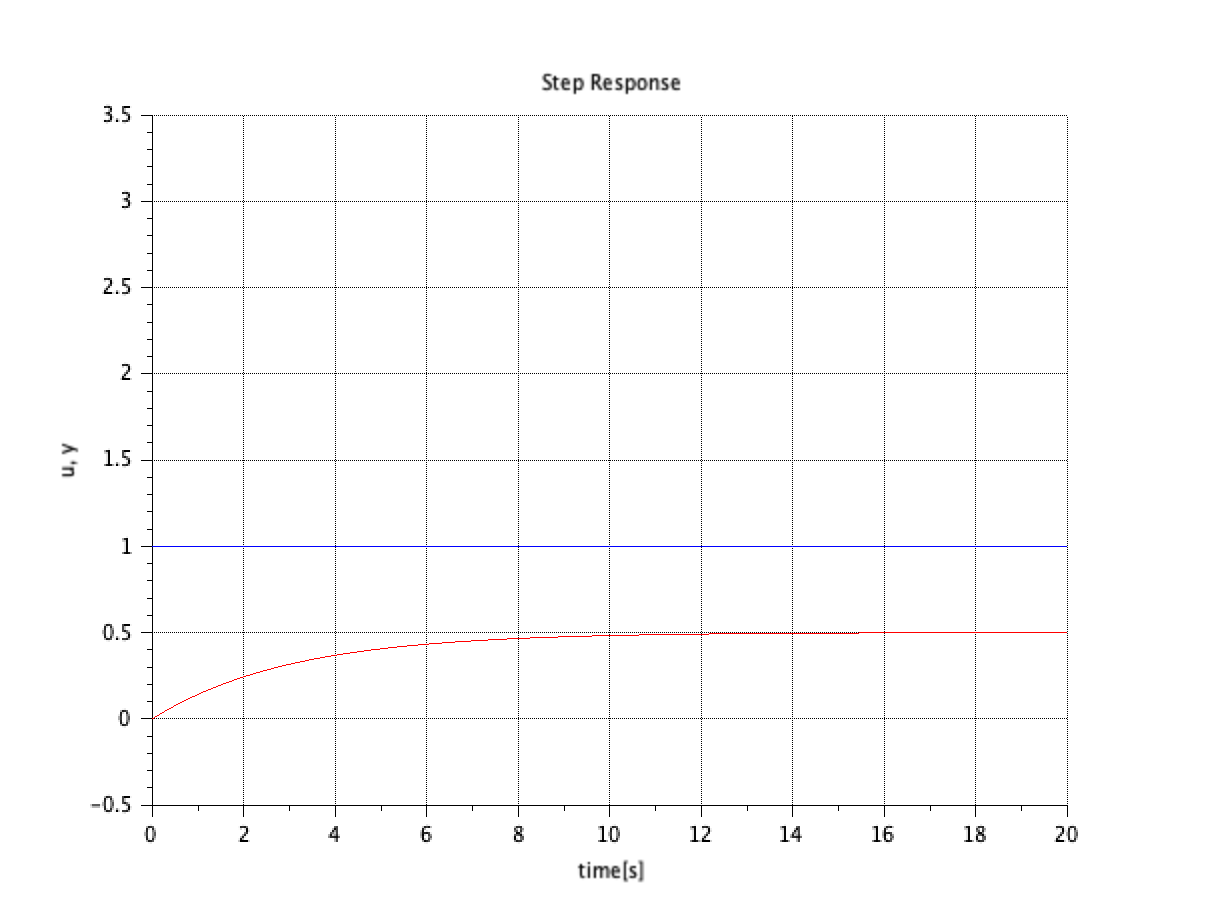
\includegraphics[clip,width=9cm]{picture/experiment1-1-4.png}
          \subcaption{$K=0.5, T=3$のときのグラフ}
          \label{G1-4}
        \end{minipage}
      \end{tabular}
      \caption{1次系伝達関数の値を変化させたグラフ}
      \label{kadai1_G}
    \end{figure}

  \subsection{2次系伝達関数}
    式\ref{2nd}に対して適当なゲイン$K$,$\omega_n$,$\zeta$を代入しグラフの変化を確認する.
    Scilabのソースコードを以下のCode\ref{code2}に示す.~\cite{text}
    \begin{lstlisting}[caption= 2次系伝達関数のソースコード, label=code2]
clear();
s = %s;
K = 1;
omega = 6;
zeta = 0.1;
P1 = syslin('c', K*omega^2/(s^2 + 2 * zeta * omega*s + omega^2));


zeta = 0.5;
P2 = syslin('c', K*omega^2/(s^2 + 2 * zeta * omega*s + omega^2));


zeta = 1.0;
P3 = syslin('c', K*omega^2/(s^2 + 2 * zeta * omega*s + omega^2));

t = 0:0.1:20;
u = ones(t);

y1 = csim(u,t,P1);
y2 = csim(u,t,P2);
y3 = csim(u,t,P3);
xmin = 0; xmax = 10; ymin = -0.5; ymax = 2;
scf(0);

plot2d(t,u,style=color(0,0,255),rect=[xmin ymin xmax ymax]);

plot2d(t,y1,style=color(255,0,0),rect=[xmin ymin xmax ymax]);
plot2d(t,y2,style=color(0,255,0),rect=[xmin ymin xmax ymax]);
plot2d(t,y3,style=color(50,0,20),rect=[xmin ymin xmax ymax]);

xtitle('Step Response', 'time[s]', 'u, y')
xgrid();
//save file as PNG
xs2png(0, 'experiment1-2.png')
    \end{lstlisting}

    また,以下の図\ref{kadai2_G}にそれぞれ値を変化させたグラフを示す.
    \begin{figure}[H]
      \begin{tabular}{cc}
        \begin{minipage}[t]{0.48\textwidth}
          \centering
          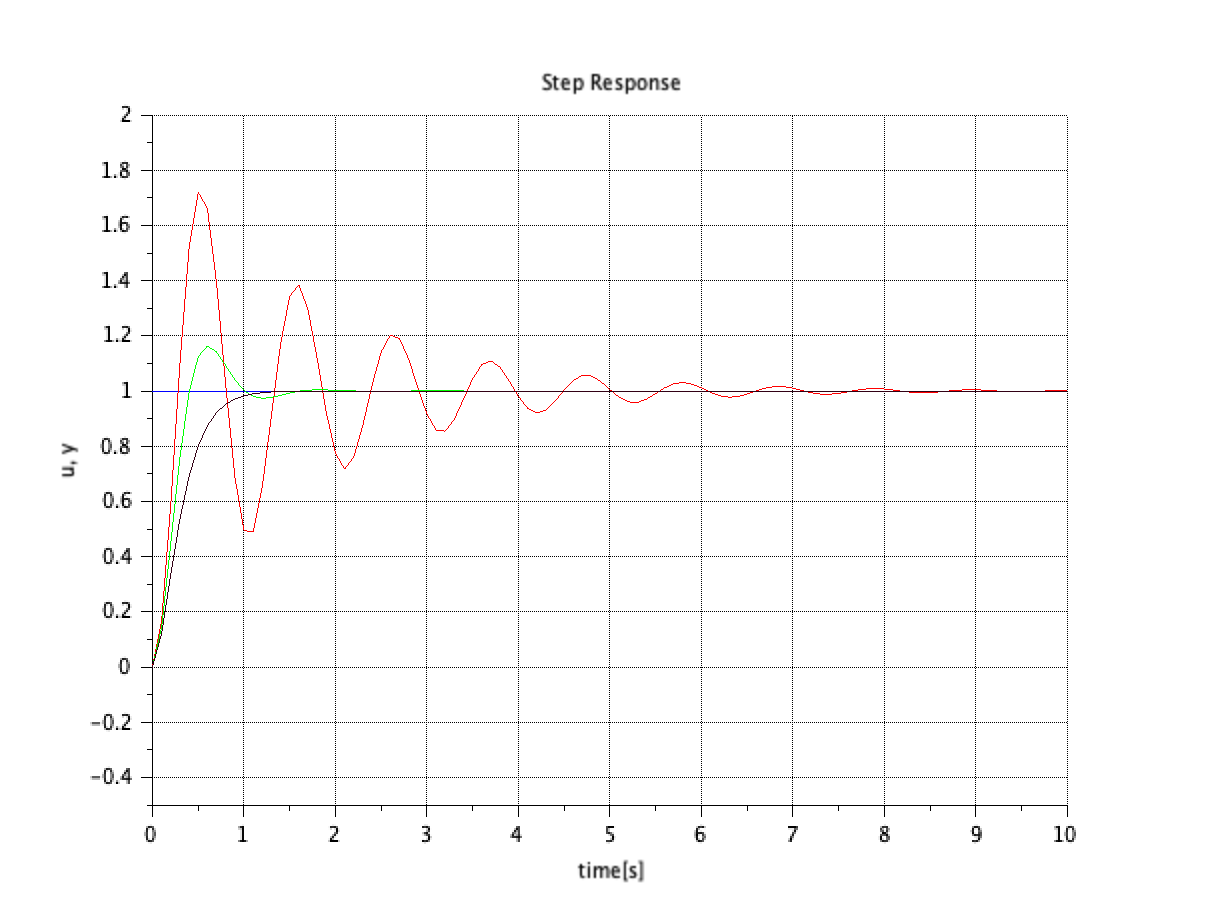
\includegraphics[clip,width=9cm]{picture/experiment1-2-1.png}
          \subcaption{$K=1, \omega_n =6, \zeta=0.1,0.5,1.0$のときのグラフ}
          \label{G2-1}
        \end{minipage} &
        \begin{minipage}[t]{0.48\textwidth}
          \centering
          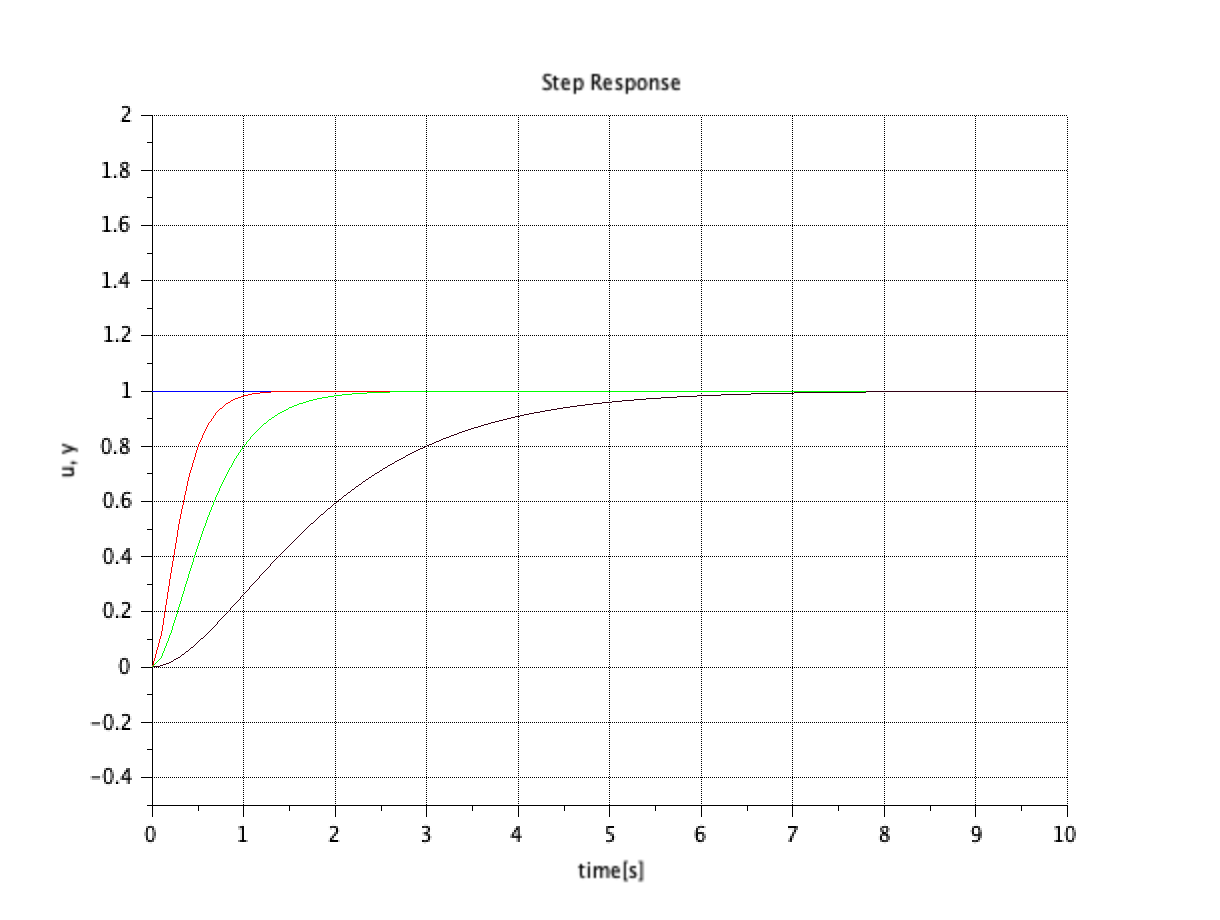
\includegraphics[clip,width=9cm]{picture/experiment1-2-2.png}
          \subcaption{$K=1, \omega_n =6,3,1, \zeta =1$のときのグラフ}
          \label{G2-2}
        \end{minipage} \\
        \begin{minipage}[t]{0.48\textwidth}
          \centering
          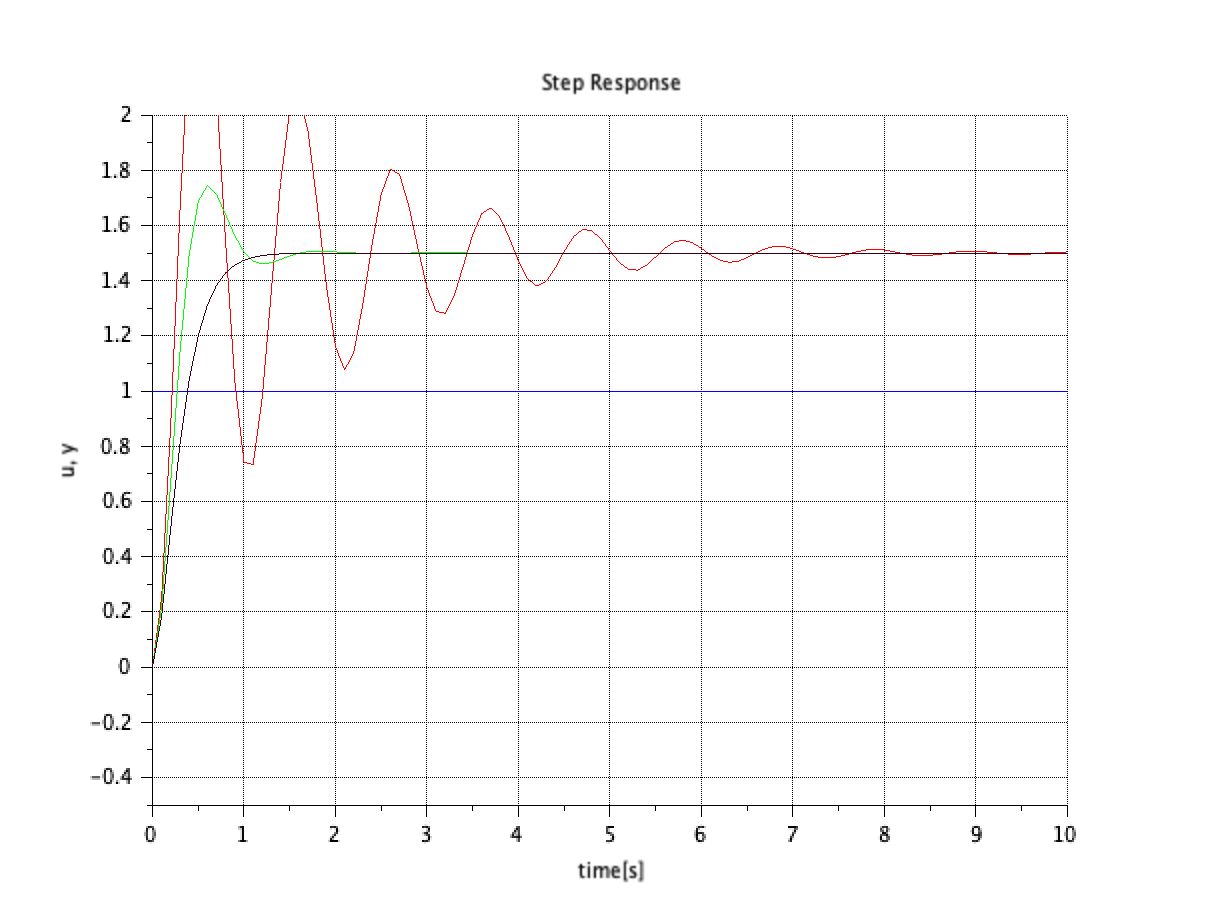
\includegraphics[clip,width=9cm]{picture/experiment1-2-3.png}
          \subcaption{$K=1.5, \omega_n = 6, \zeta = 0.1,0.5,1.0$のときのグラフ}
          \label{G2-3}
        \end{minipage} &
        \begin{minipage}[t]{0.48\textwidth}
          \centering
          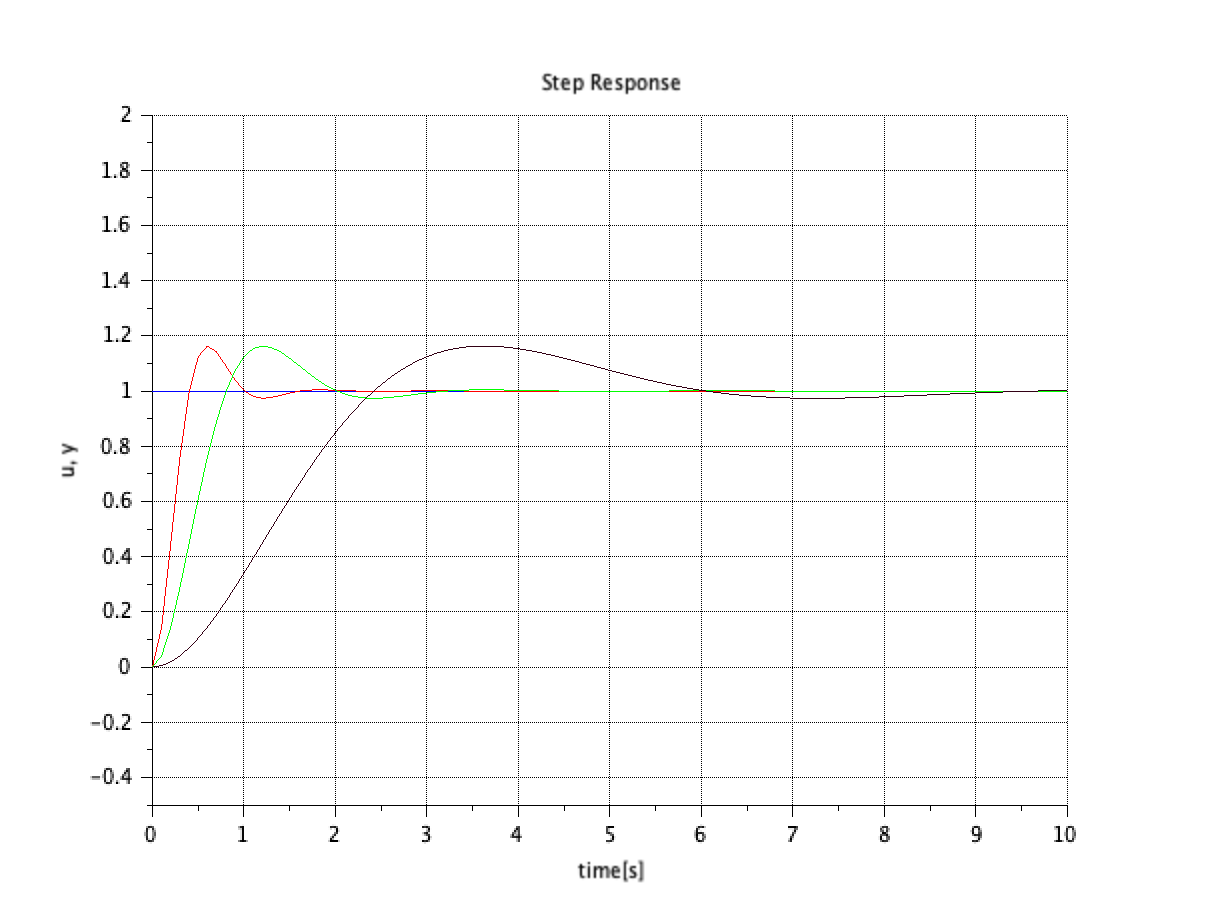
\includegraphics[clip,width=9cm]{picture/experiment1-2-4.png}
          \subcaption{$K=1, \omega_n =6,3,1, \zeta =0.5$のときのグラフ}
          \label{G2-4}
        \end{minipage}
      \end{tabular}
      \caption{2次系伝達関数の値を変化させたグラフ}
      \label{kadai2_G}
    \end{figure}

  \subsection{研究課題}
    \begin{quote}
      実験1において,SIMULINKシミュレーションのサンプル時間を0.001[sec]から1[sec]まで変化
      させたときの計算結果を比較し,考察しなさい.
    \end{quote}
    以下に研究課題の実行結果を示す.ここで,Scilabではソースコード\ref{code1}を使用し,$K=3,T=1$
    を代入している.サンプル時間は$t=0:1:20$(図\ref{ex1})と$t=0:0.001:20$(図\ref{ex2})で比較しており,比較しやすいように,x軸の表示範囲
    を$0\sim 10$に変更している.
    \begin{figure}[H]
      \begin{tabular}{cc}
        \begin{minipage}[t]{0.48\textwidth}
          \centering
          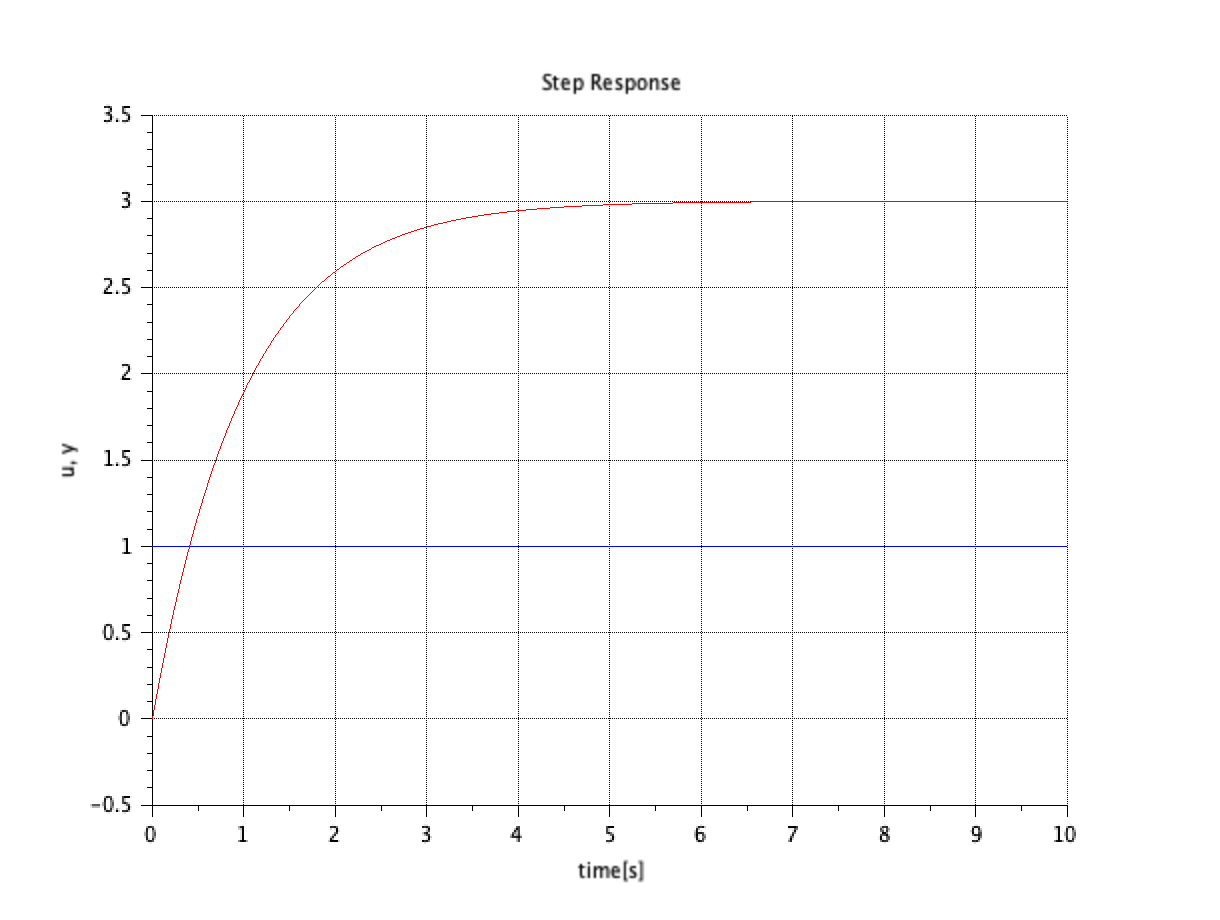
\includegraphics[clip,width=9cm]{picture/ex1.png}
          \caption{$t=0:0.001:20$のグラフ}
          \label{ex1}
        \end{minipage} &
        \begin{minipage}[t]{0.48\textwidth}
          \centering
          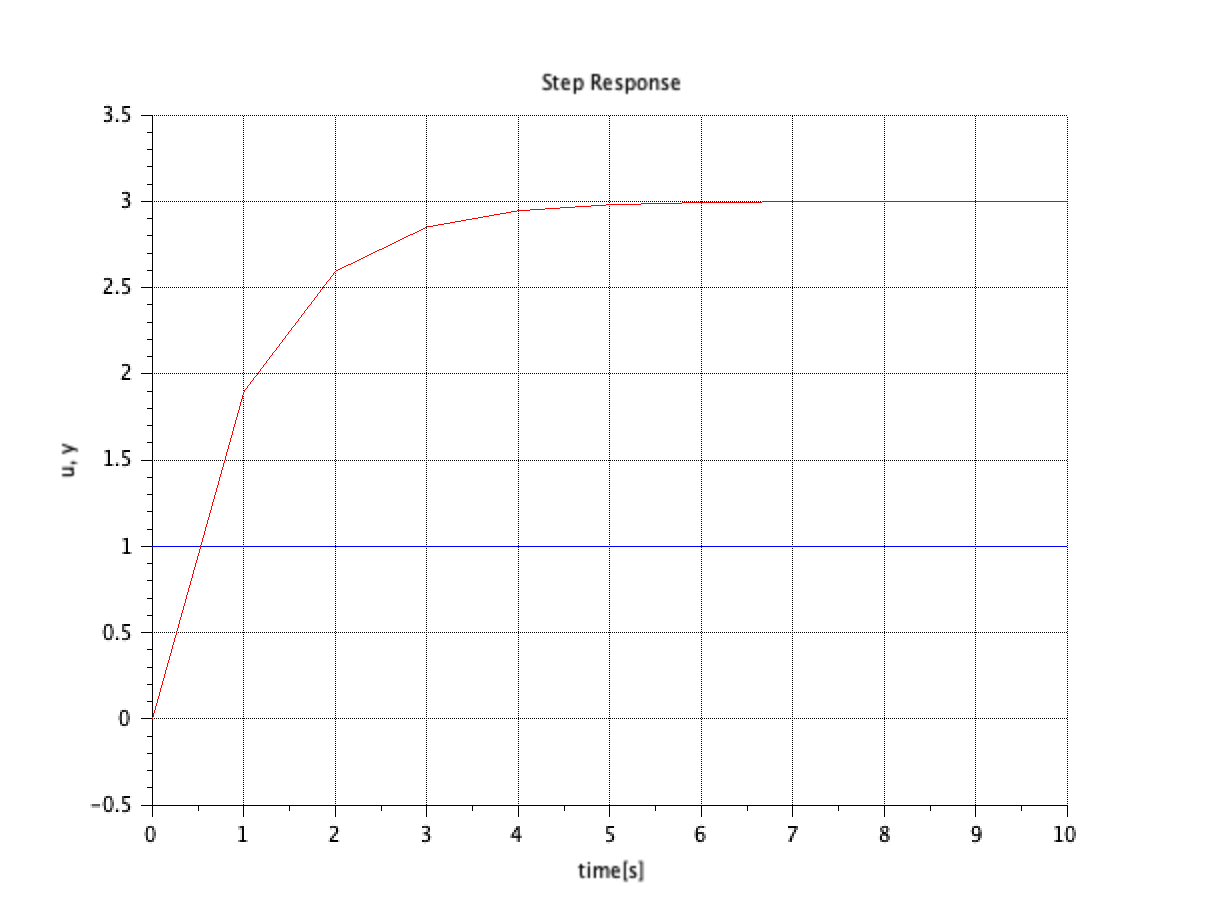
\includegraphics[clip,width=9cm]{picture/ex2.png}
          \caption{$t=0:1:20$のグラフ}
          \label{ex2}
        \end{minipage}
      \end{tabular}
    \end{figure}

  \section{考察}
    研究課題において,サンプル時間を変更したことでなめらかなグラフとカクカクしたグラフを
    出力することができた.これはサンプル時間が小さくなるほど図\ref{ex1}のような精度の高いグラフを出力することが
    できることを表しており,図\ref{ex2}のようなグラフは精度が低いと言える.
    したがって,正しい数値をグラフから読み取るためには,十分なサンプルを取得しグラフを出力することが
    大切である.

\begin{thebibliography}{3}
  \bibitem{ESI} ESI-Grope "Scilab/Xcosとは(1)" (最終閲覧日 2021年5月16日)\\\url{https://solution.esi.co.jp/scilab/blog/introduction1}
  \bibitem{kato} Joseph Edminister,Mahmood Nahvi "Electric Circuits, 6th edition" (出版年 2013/11/8)
  \bibitem{text} 永田 正伸 "制御系CAD:Scilabによる過渡応答シュミレーション" 制御情報システム工学科 制御工学実験 指導書 2020.6
\end{thebibliography}


\end{document}